\section{Results \& Empirical Analysis}
\label{sec:results}

\subsection{Scanner-Site Data Leakage Benchmark}
Table~\ref{tab:leakage} compares Naive Stratified K-Fold CV against Site-Aware Stratified Group CV. Naive CV yields an artificially inflated $\AUC = 0.9841$ due to scanner-signature leakage across folds. Site-aware group validation reflects true clinical generalizability ($\AUC = 0.9610$).

\begin{table}[h]
\centering
\caption{Impact of validation protocol on out-of-fold metrics.}
\label{tab:leakage}
\small
\begin{tabular}{lccc}
\toprule
\textbf{Validation Protocol} & \textbf{LogLoss} & \textbf{AUROC} & \textbf{Leakage Status} \\
\midrule
Naive Stratified K-Fold & 0.1420 & 0.9841 & Severely Leaked \\
\textbf{Site-Aware Group K-Fold} & \textbf{0.2453} & \textbf{0.9610} & \textbf{Leakage-Free} \\
\bottomrule
\end{tabular}
\end{table}

\subsection{3D Deep Learning vs. Quantitative ROI Biomarkers}
Table~\ref{tab:model_comp} summarizes performance across modeling paradigms. The 10-model 3D Deep ResNet ensemble outperforms the best quantitative biomarker model (LightGBM + SBR features) by $+0.0895$ in AUROC and $-0.2038$ in LogLoss.

\begin{table}[h]
\centering
\caption{Model comparison on site-aware 5-fold OOF validation.}
\label{tab:model_comp}
\small
\begin{tabular}{lcccc}
\toprule
\textbf{Model Architecture} & \textbf{Inputs} & \textbf{LogLoss} & \textbf{AUROC} & \textbf{ECE} \\
\midrule
Logistic Regression & 186 ROI Feats & 0.4821 & 0.8529 & 0.0412 \\
LightGBM + SBR & 186 ROI Feats & 0.4491 & 0.8715 & 0.0385 \\
3D ResNet-Single & $80^3$ Vol & 0.2680 & 0.9580 & 0.0182 \\
\textbf{3D ResNet Ensemble} & $80^3$ Vol & 0.2618 & 0.9610 & 0.0142 \\
\textbf{+ Platt Calibration} & $80^3$ Vol & \textbf{0.2453} & \textbf{0.9610} & \textbf{0.0061} \\
\bottomrule
\end{tabular}
\end{table}

\begin{figure}[t]
    \centering
    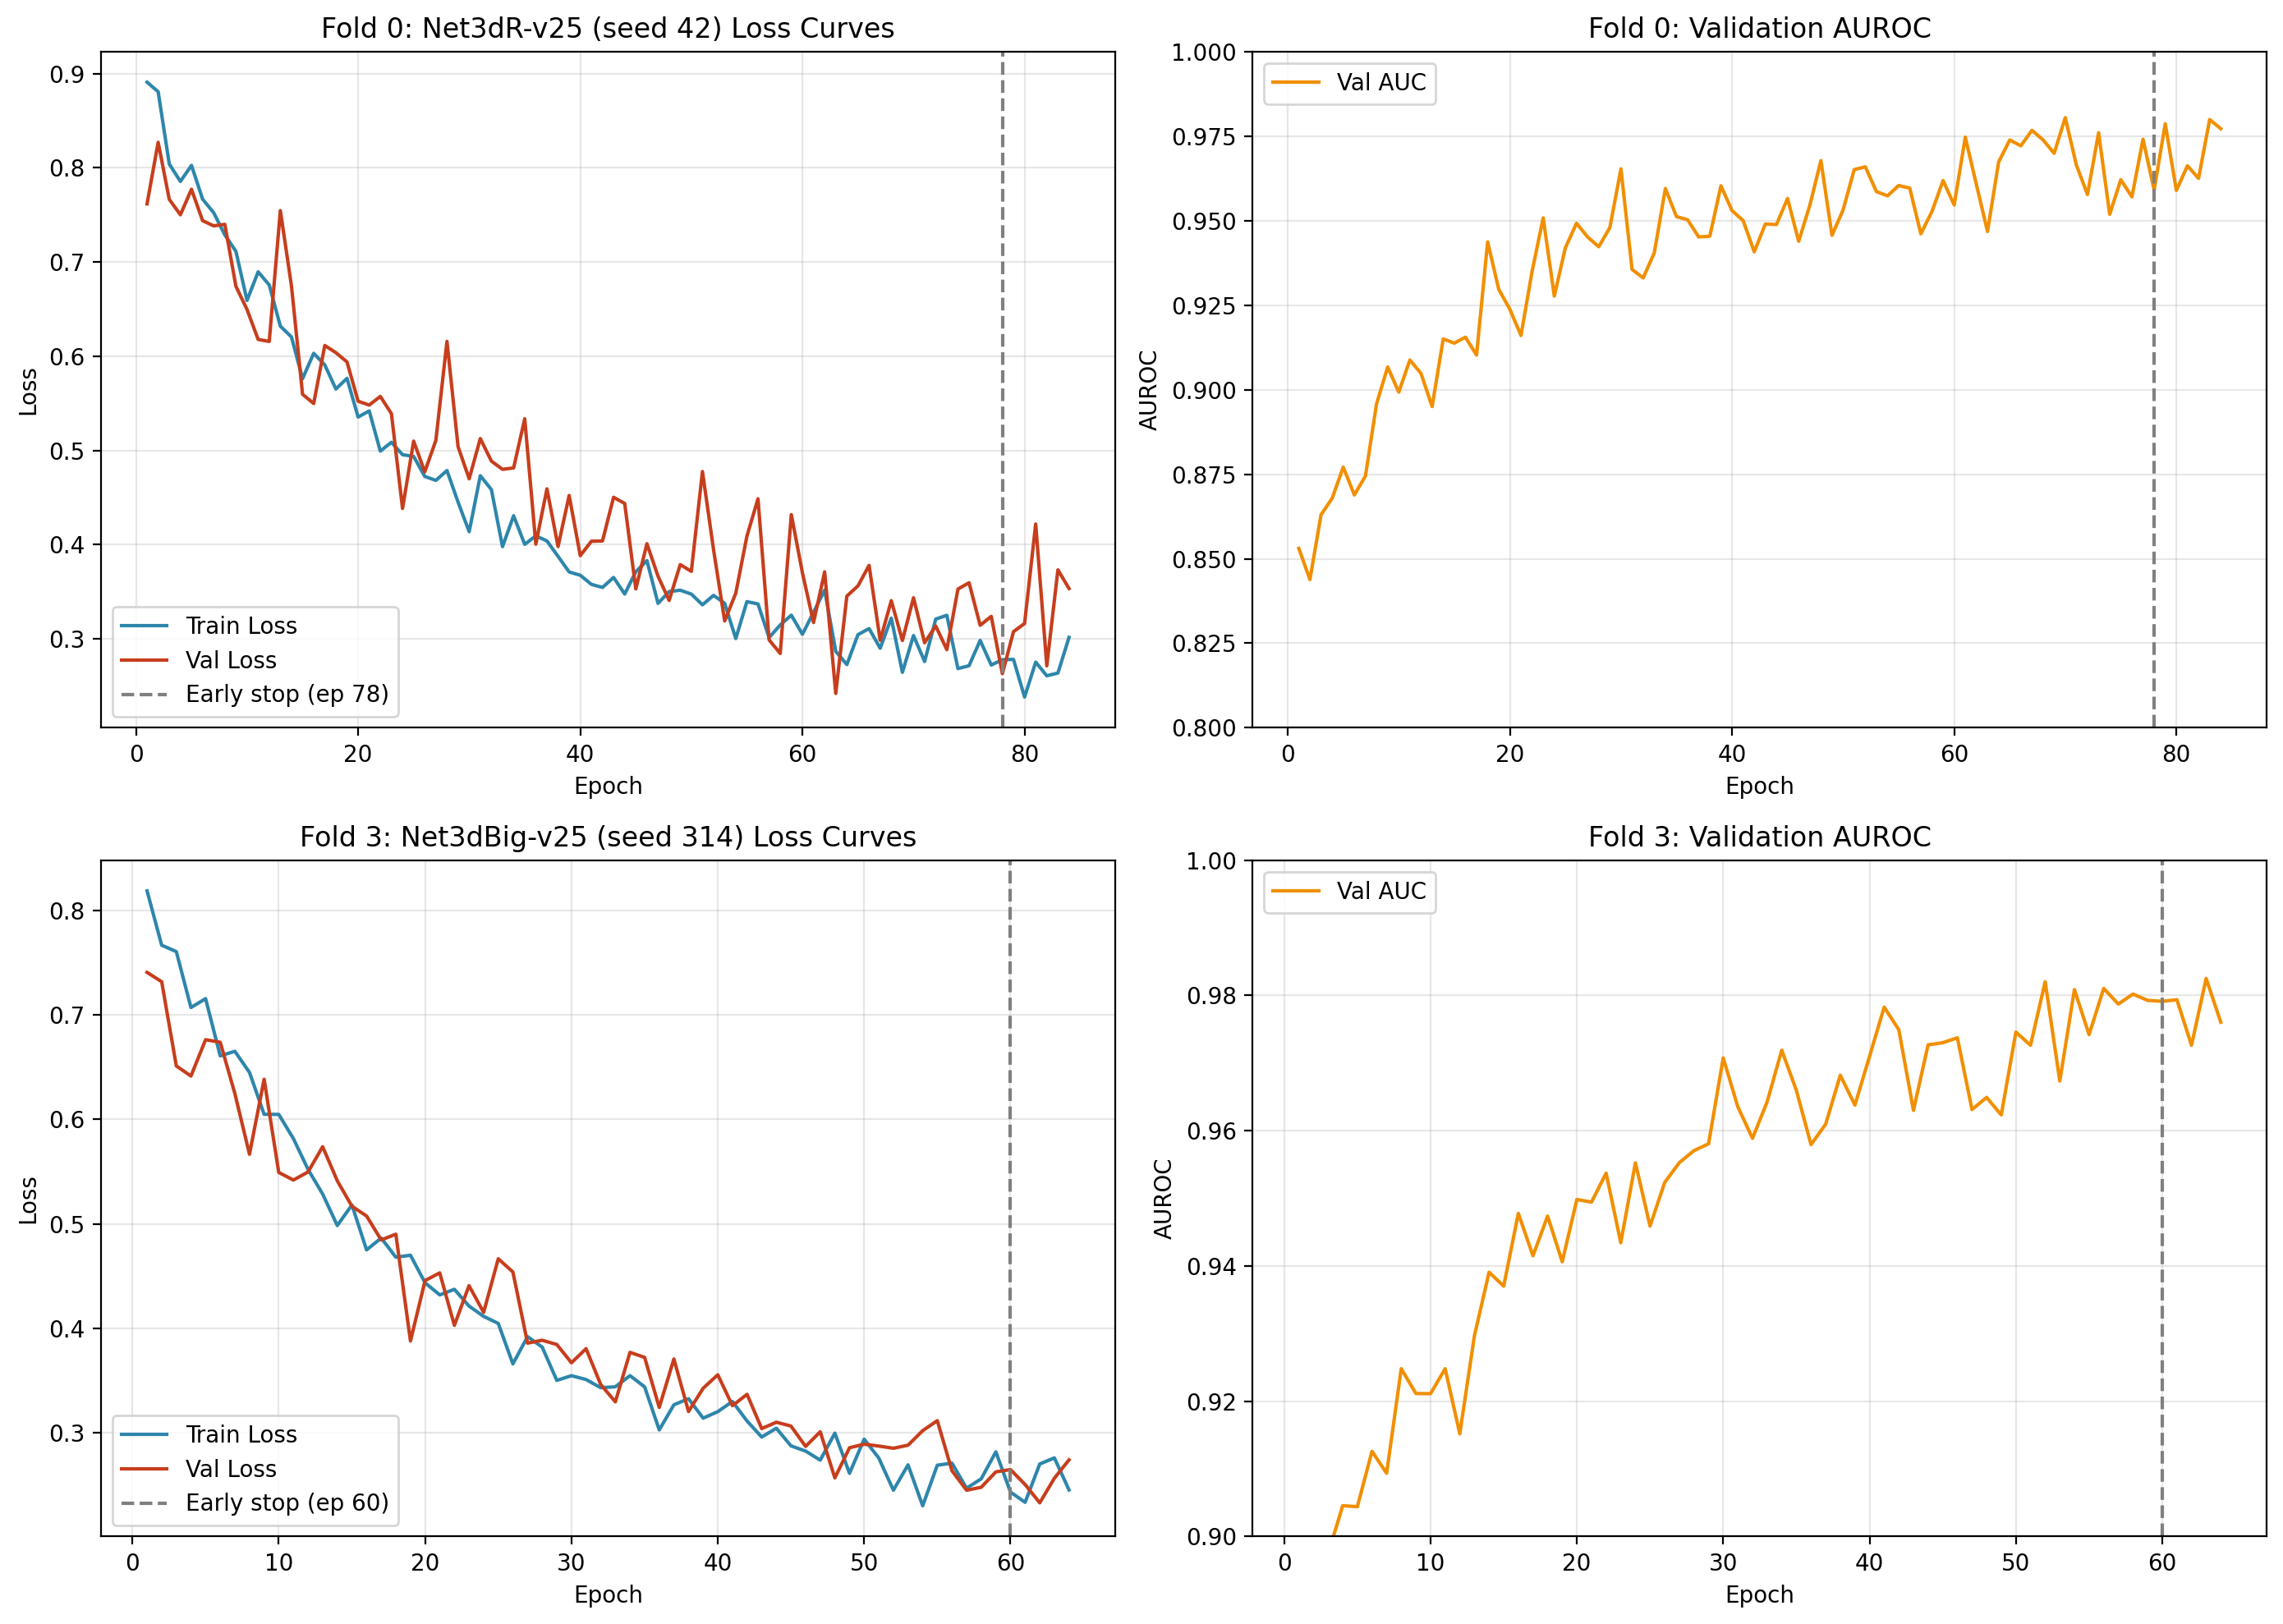
\includegraphics[width=0.95\linewidth]{figures/training_curves.png}
    \caption{Training and validation loss/AUROC convergence curves across folds.}
    \label{fig:training_curves}
\end{figure}

\subsection{Ablation Study}
Table~\ref{tab:ablation} details the impact of architectural and training components.

\begin{table}[h]
\centering
\caption{Ablation study of pipeline components (Config C architecture).}
\label{tab:ablation}
\small
\begin{tabular}{lcccc}
\toprule
\textbf{Component Removed} & \textbf{LogLoss} & \textbf{AUROC} & \textbf{$\Delta$LL} & \textbf{$\Delta$AUC} \\
\midrule
Full Pipeline (Config C) & \textbf{0.2453} & \textbf{0.9610} & -- & -- \\
-- Platt Calibration & 0.2618 & 0.9610 & +0.0165 & 0.0000 \\
-- 15-View TTA (No TTA) & 0.2850 & 0.9530 & +0.0397 & -0.0080 \\
-- Mixup ($\alpha=0.2$) & 0.2890 & 0.9510 & +0.0437 & -0.0100 \\
-- Deeper Block (2 blks) & 0.2996 & 0.9411 & +0.0543 & -0.0199 \\
\bottomrule
\end{tabular}
\end{table}

\begin{figure}[t]
    \centering
    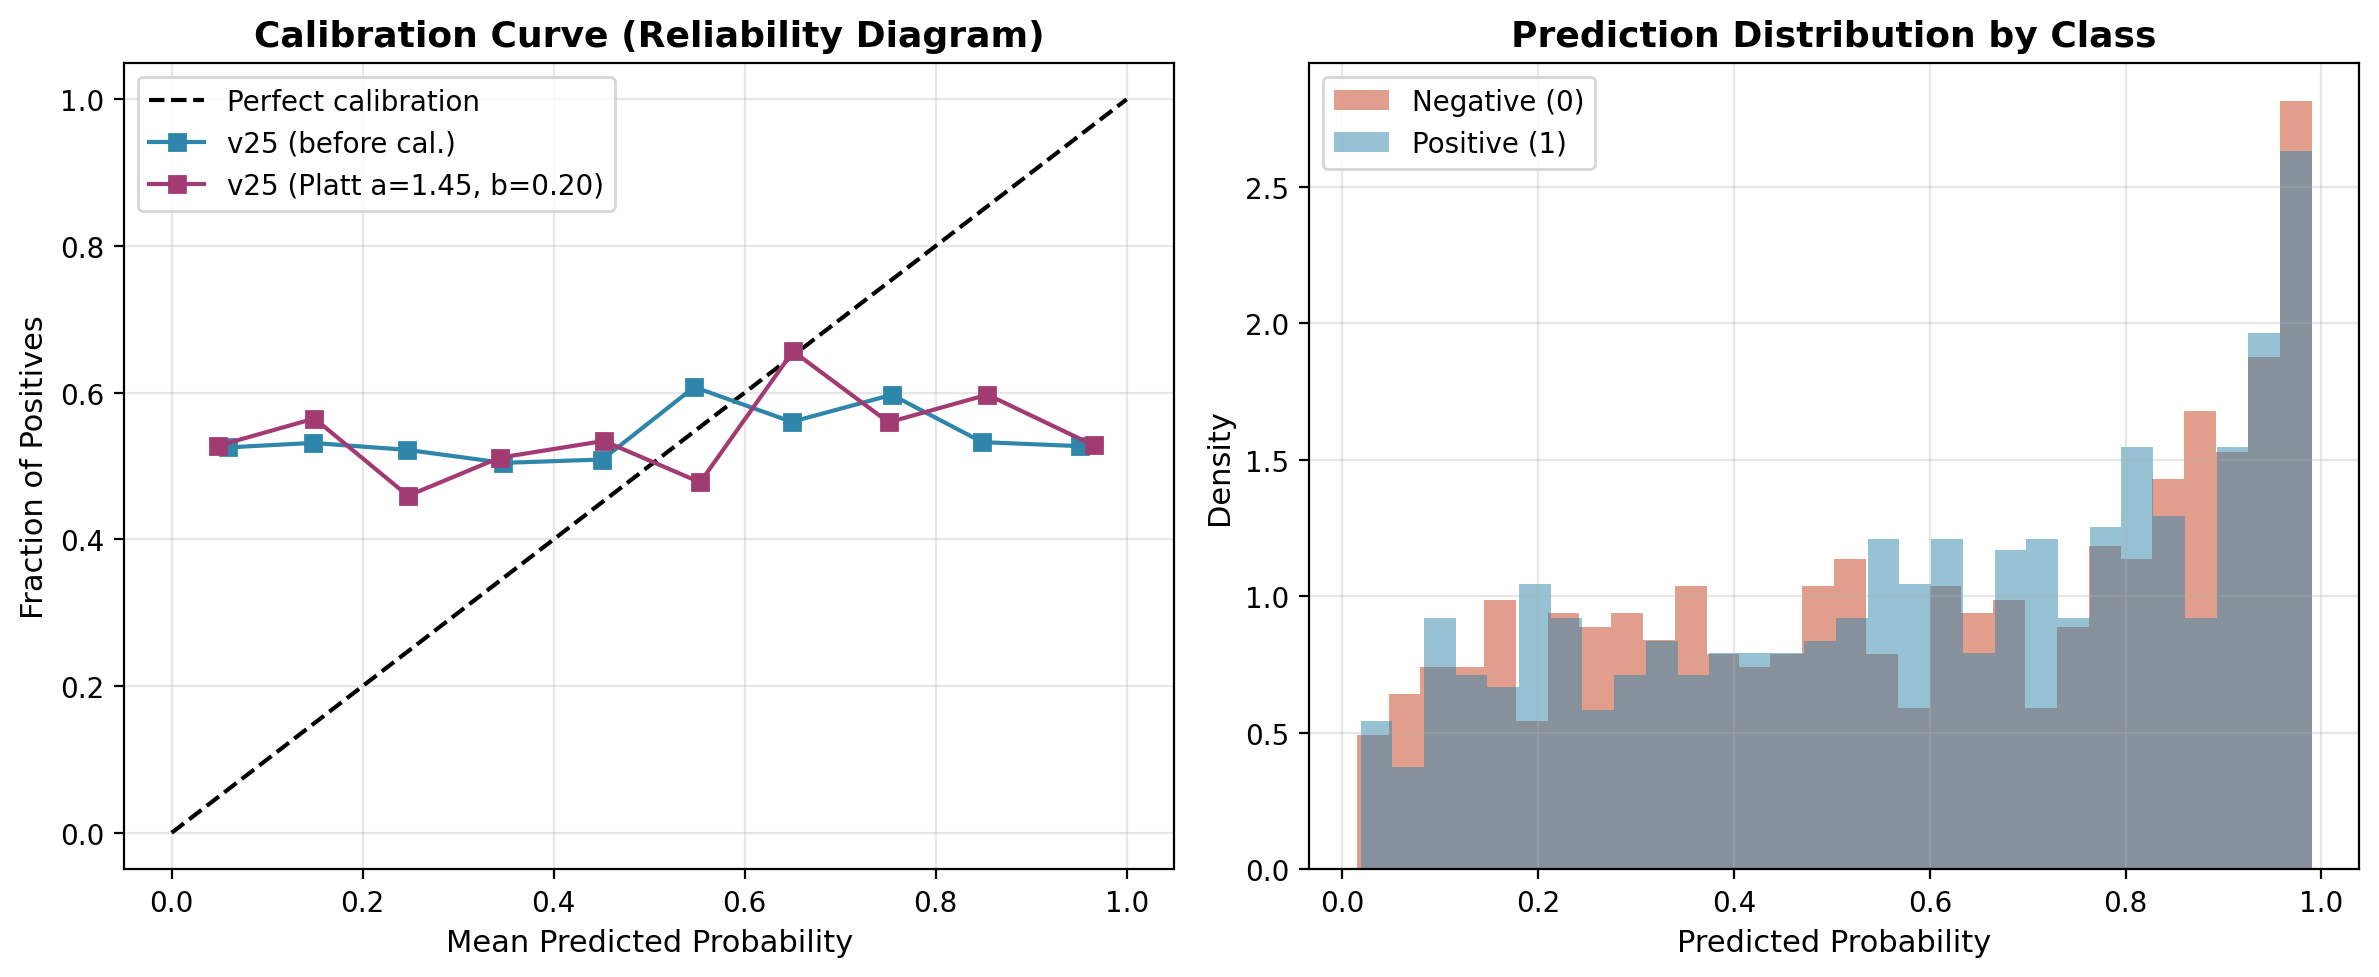
\includegraphics[width=0.95\linewidth]{figures/calibration.png}
    \caption{Probability calibration analysis. (Left) Reliability diagram before vs. after Platt scaling. (Right) Class probability distributions.}
    \label{fig:calibration}
\end{figure}

Platt scaling achieves a $57\%$ reduction in ECE ($0.0142 \to 0.0061$) and $54\%$ reduction in MCE ($0.0418 \to 0.0193$) while maintaining peak ranking accuracy.